\chapter{Electrmagnetic Waves}

\section{Light}
Light is electromagnetic radiation, figure \ref{fig:spectrum} shows the 
spectre of EM radiation. 

\begin{figure}[h!]
    \centering
    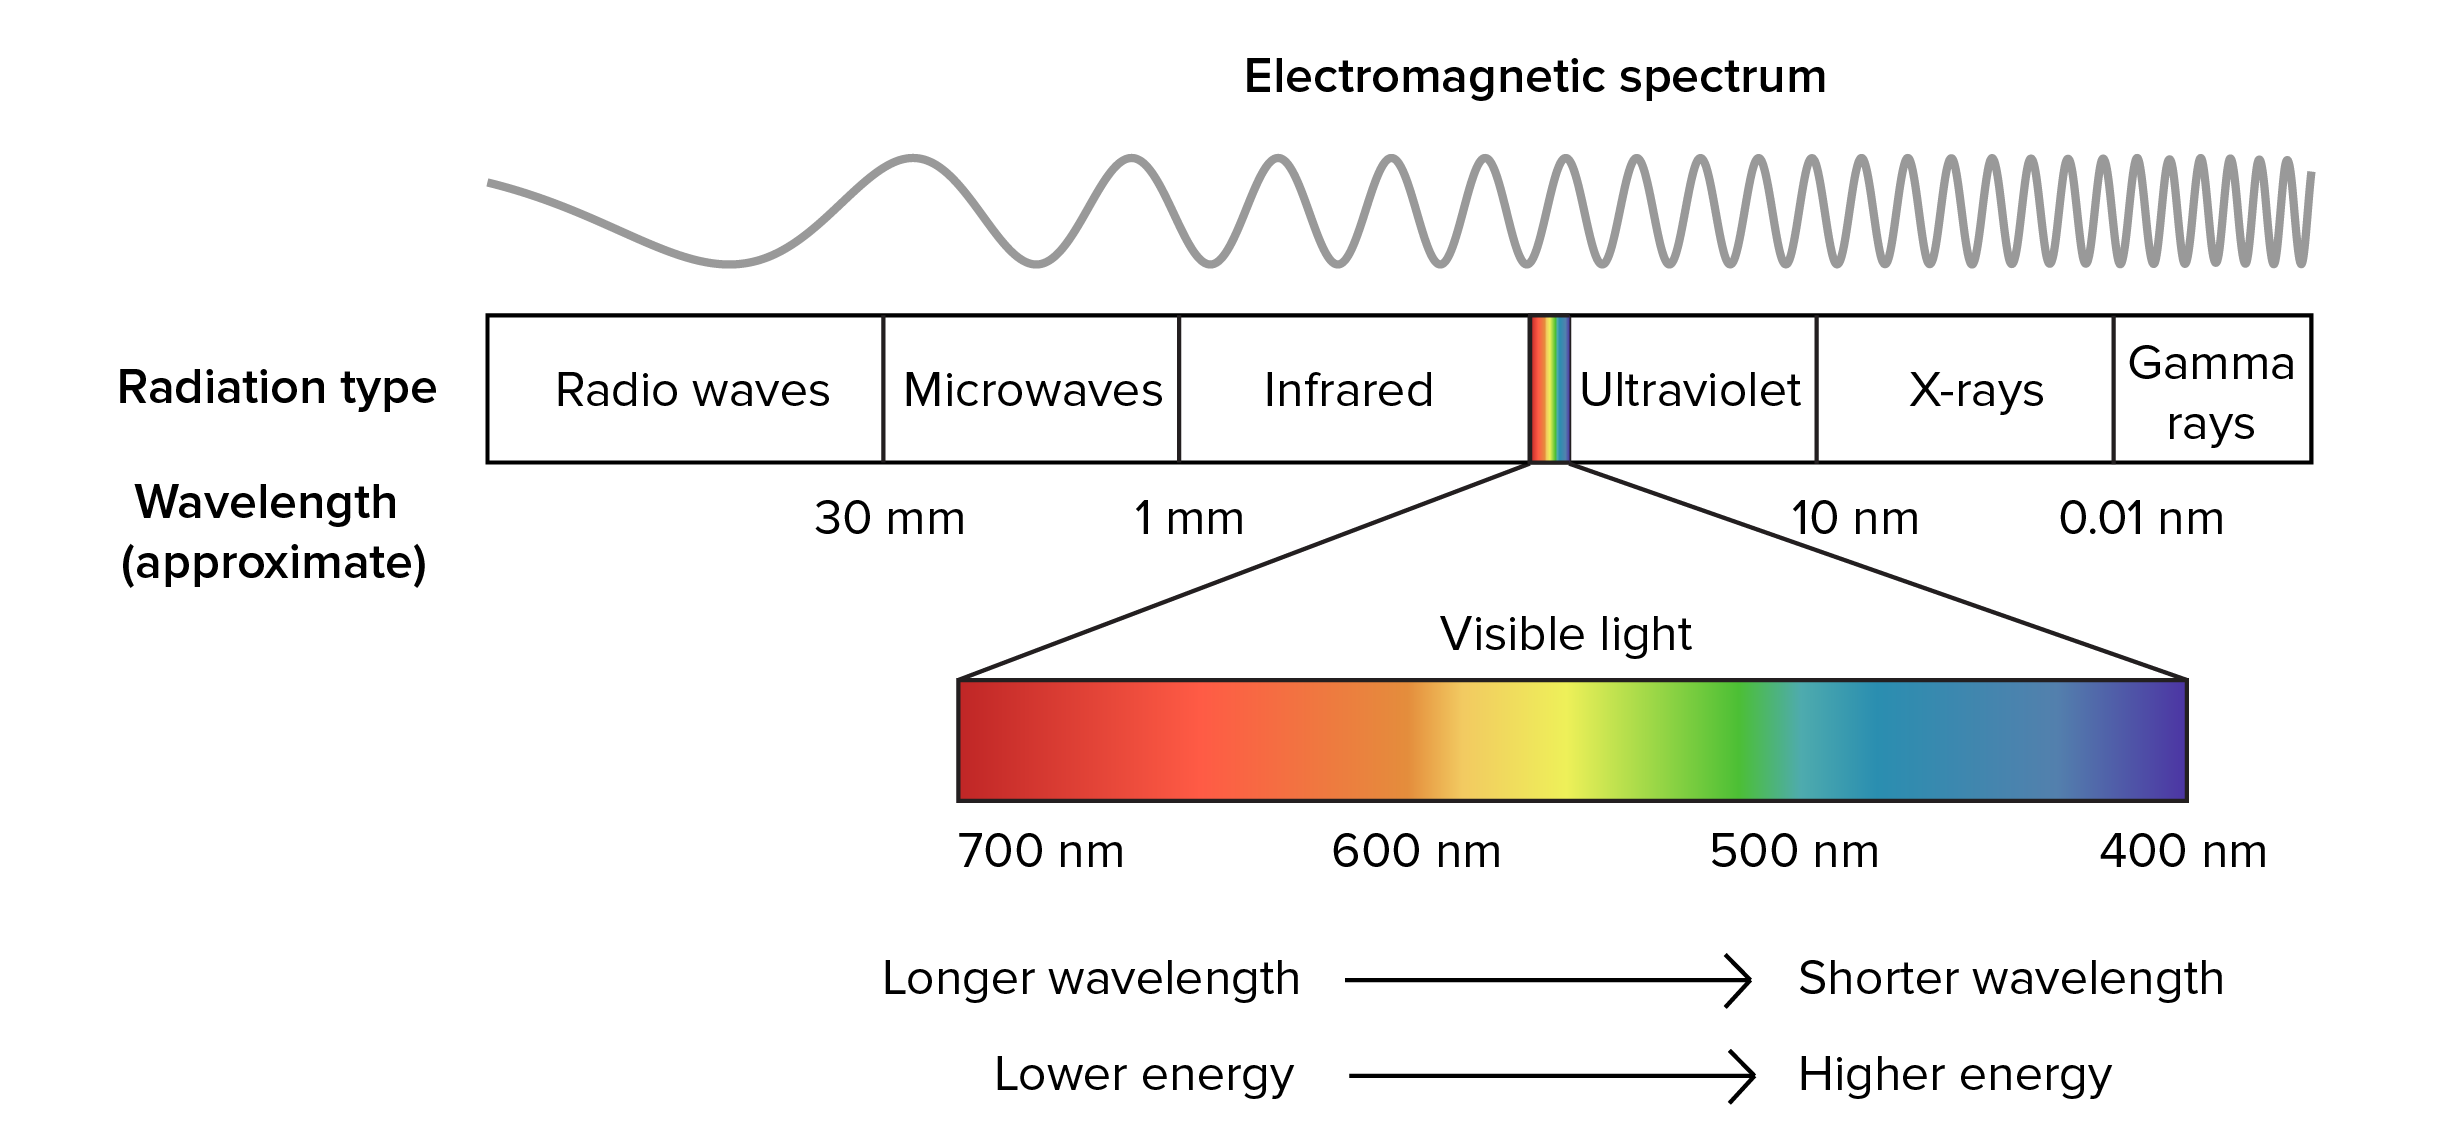
\includegraphics[width=0.5\textwidth]{slike/spectrum.png}
    \caption{Spectrum of EM}
    \label{fig:spectrum}
\end{figure}

Light of one wavelength can be described by the equation \ref{eq:light1}.
\begin{equation}
    \nu \cdot \lambda = c
    \label{eq:light1}
\end{equation}
Where $\nu$ is the frequency, $\lambda$ is the wavelength and $c$ the speed of
light. 
Speed of light is equal to $c \approx 3 \cdot 10^8 \frac{m}{s}$.

\section{Electromagnetic radiation}
An example source of EM radiation - dipole radiation -  is an oscillating electron, at a certain frequency and amplitude.
Close to the source we can describe the EM field using the \textit{Faraday's law}, equation \ref{eq:fl}.
\begin{equation}
    \nabla \times E  = - \frac{\partial B}{\partial t}
    \label{eq:fl}
\end{equation}
Where $E$ is the electric field and $B$ is the magnetic field.

Magnetic and electric fields are perpendicular to each other, as shown on figure \ref{fig:mef}.
\begin{figure}[h!]
    \centering
    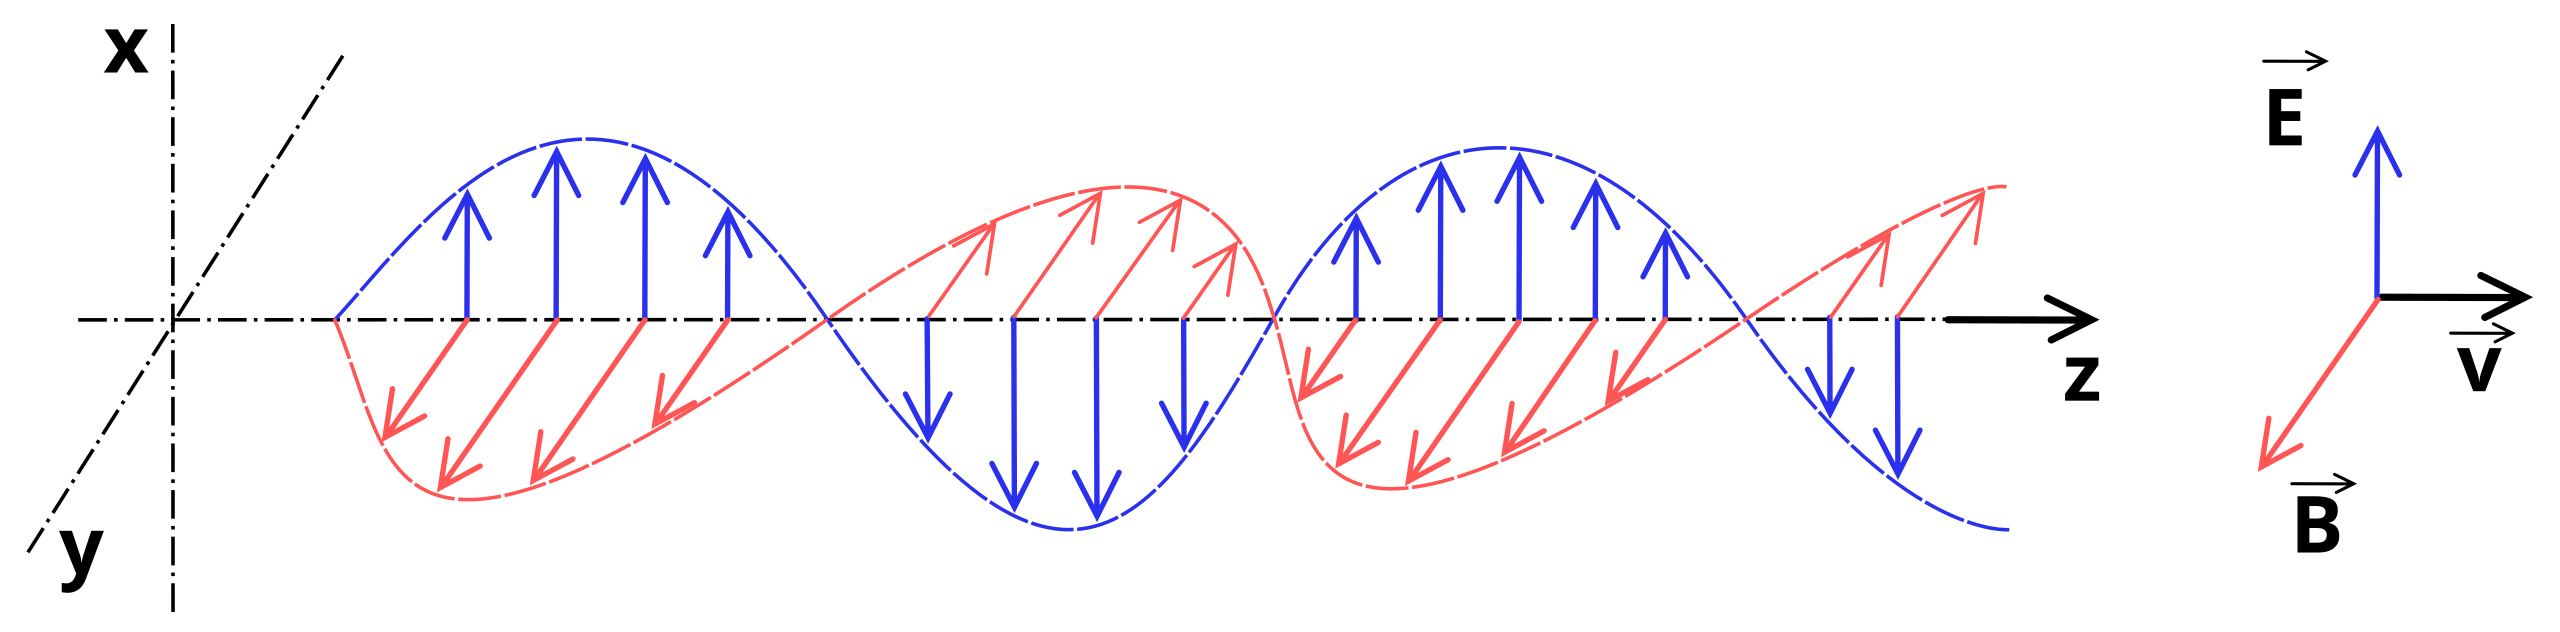
\includegraphics[width=0.5\textwidth]{slike/Onde_electromagnetique.svg.png}
    \caption{Magnetic and electric field}
    \label{fig:mef}
\end{figure}

Far from the origin, EM field is \textbf{perpendicular to propagation direction}.
Electric field and magnetic fields are synchronized and perpendicular. These two simplifications,
neglect field directions and only consider $E$ and $B$ fields along the propagation directions.
Consequences of this are:
\begin{enumerate}
    \item Loose information about 3D shape of radiation
    \item \textbf{Much simpler mathematical description}
\end{enumerate}



In summary - properties of EM-waves are:
\begin{itemize}
    \item is generated by dipole moment change
    \item electric and magnetic fields are synchronized and point towards orthogonal directions, both fields are perpendicular to the propagation direction $\rightarrow$ transverse wavelength
    \item electric and magnetic filed directions depend on the oscillation directions dependent on the oscillation orientation of the dipole $\rightarrow$ polarization
    \item oscillation frequency of the dipole determines the wavelength
\end{itemize}


\subsection{EM-wave in one dimension}
\begin{figure}[h!]
    \centering
    \includegraphics[width=0.5\textwidth]{slike/simplewave.pdf}
    \caption{Simple wave}
    \label{fig:simplewave}
\end{figure}

Where $\lambda$ is the wavelength, $A_0$ is the filed strength (amplitude), $\varphi$ is the phase delay or shift. 
From this, we can derive  wave number \ref{eq:wavenumber}:

\begin{equation}
    k = \frac{2 \pi}{\lambda}
    \label{eq:wavenumber}
\end{equation}
Angular frequency, \ref{eq:angfreq}:
\begin{equation}
    \omega = 2 \pi \nu
    \label{eq:angfreq}
\end{equation}

Using \ref{eq:angfreq} and \ref{eq:wavenumber}, we can derive \ref{eq:wave}:
\begin{equation}
    A(x,t) = A_0 cos(kx - \omega t + \varphi)
    \label{eq:wave}
\end{equation}

\subsection{EM-wave in 3D}
To describe the wave in 3D space, we can use equation \ref{eq:w3d}.
\begin{equation}
    \vec{A}(\vec{r},t) = \vec{A}_0 cos(\vec{k} \cdot \vec{r} - \omega t + \varphi)
    \label{eq:w3d}
\end{equation}

Where $A_0$ is a field vector - direction of EM-field, $\vec{r}$ is position vector in space, 
$\vec{k}$ is the wave vector - points along the propagation direction ($k_x$,$k_y$,$k_z$).
\textbf{Dot product} $\vec{k} \cdot \vec{r}$ is a constant - mathematical definition of a plane.
Figure \ref{fig:linplw} shows the linear plane wave in 3D.
%https://en.wikipedia.org/wiki/Sinusoidal_plane_wave

\begin{figure}[h!]
    \centering
    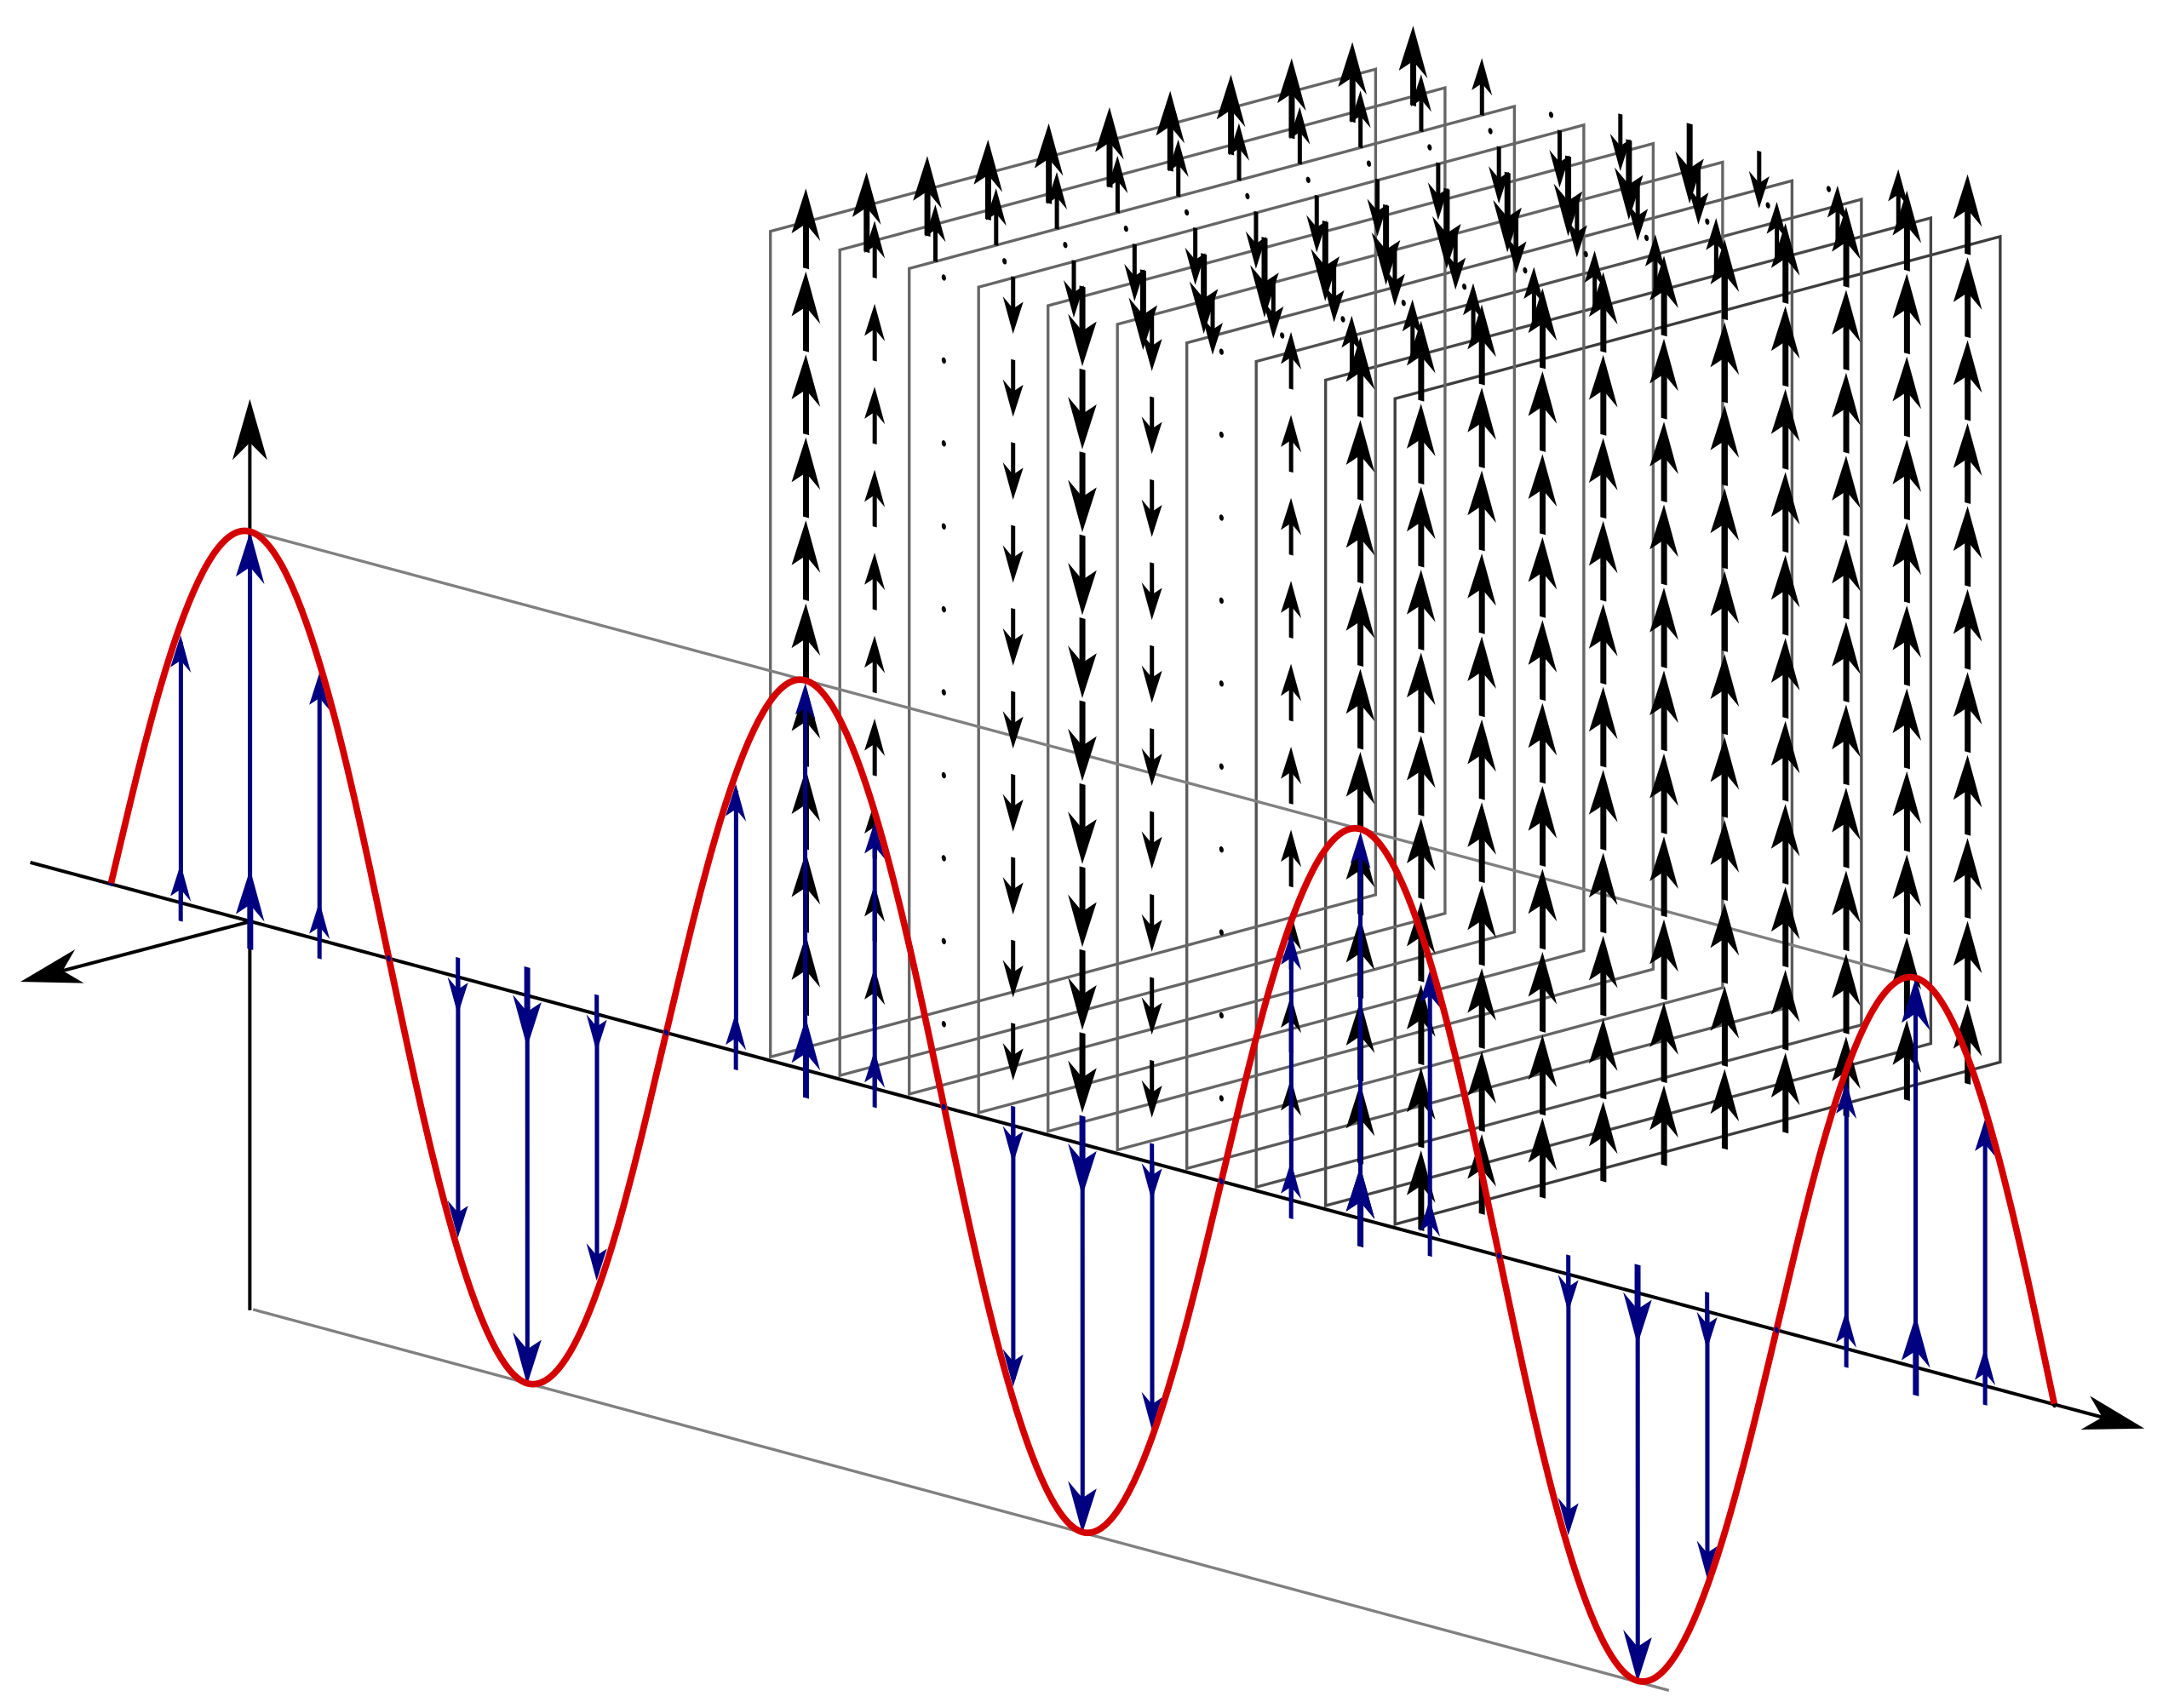
\includegraphics[width=0.4\textwidth]{slike/linplanewave.png}
    \caption{Linear plane wave}
    \label{fig:linplw}
\end{figure}

We use simplifications for describing the plane wave, its wavefronts are:
\begin{itemize}
    \item  parallel
    \item  infinite
    \item  orthogonal to propragation direction
\end{itemize}
True plane-waves do not exist, they are a convenient mathematical tool.



\section{Power and intensity}
Electric and magnetic fields store energy according to equation \ref{eq:ed}.
\begin{equation}
    u_{EM} = \frac{\varepsilon}{2} |E|^2 + \frac{1}{2\mu} |B|^2
    \label{eq:ed}
\end{equation}
Where $\varepsilon$ is permittivity of medium, $\varepsilon = \varepsilon_R \varepsilon_0$
and $\mu$ is magnetic permeability, $\mu = \mu_R \mu_0$. $\varepsilon_0$ is equal to $8.854 \cdot 10^{-12} \frac{F}{m}$.
$\mu = 1.256 \cdot 10^{-6} \frac{N}{A^{2}}$.
Figure \ref{fig:EBwave} show a diagram of a wave. At the intersections of $E$ and $B$ fields
- crossings, power is equal to zero (Green circles). This is hard to measure.
\begin{figure}[h!]
    \centering
    \includegraphics[width=0.5\textwidth]{slike/EBfield.pdf}
    \caption{E and B wave with zero crossings}
    \label{fig:EBwave}
\end{figure}

Although there is no energy in the crossings, for most practical applications
we still consider that there is \textbf{continuous energy flow}. 
We introduce \textbf{power} and \textbf{intensity}. 
Power $P = \frac{\Delta E}{\Delta t}$ and intensity is equal to $\frac{Powe}{Area}$. 
For a plane wave intensity is calculated as \ref{eq:pd}, where $n$ is the refractive index, $c$ is the speed of light and $\varepsilon_0$ is vacuum 
permittivity. 

\begin{equation}
    I = \frac{c n \varepsilon_0}{2} |E|^2
    \label{eq:pd}
\end{equation}

\subsection{Power and energy}
Power is equal to $\frac{Energy}{Time}$, unit is Watt - $W = \frac{J}{s}$.
Average power is $P = \frac{\Delta E}{\Delta t}$ and instantaneous power is $P = \frac{dE}{dt}$.
Average intensity $I = \frac{\Delta P}{\Delta A}$  and local intensity is $I = \frac{d P}{d A}$

\section{Polarization}

Polarization of an electromagnetic wave is given ny the \textbf{orientation of its electric component}. Because the magnetic field $B$ is 
negligible compared to the electric field, for polarization of light, we will \textbf{only use} $\vec{E}$.

Polarization is important due to:
\begin{itemize}
    \item Brewster angle - optical components, absorption efficiency
    \item Processing effects - laser introduced surface structures
    \item Focusing quality
    \item Birefringence effects - focus quality degradation, wavelength conversion
\end{itemize}

\subsection{Brewster angle}
Brewster angle is an angle of incidence at which light with certain polarization is 
perfectly transmitted through a transparent dielectric surface, with no reflection.
Brewster's angle is calculated as \ref{eq:brewstr}. 

\begin{equation}
    \theta_B = arctan(\frac{n_2}{n_1})
    \label{eq:brewstr}
\end{equation}

Figure \ref{fig:brewstr} show the light interacting with two different mediums, with different $n$.
\begin{figure}[h!]
    \centering
    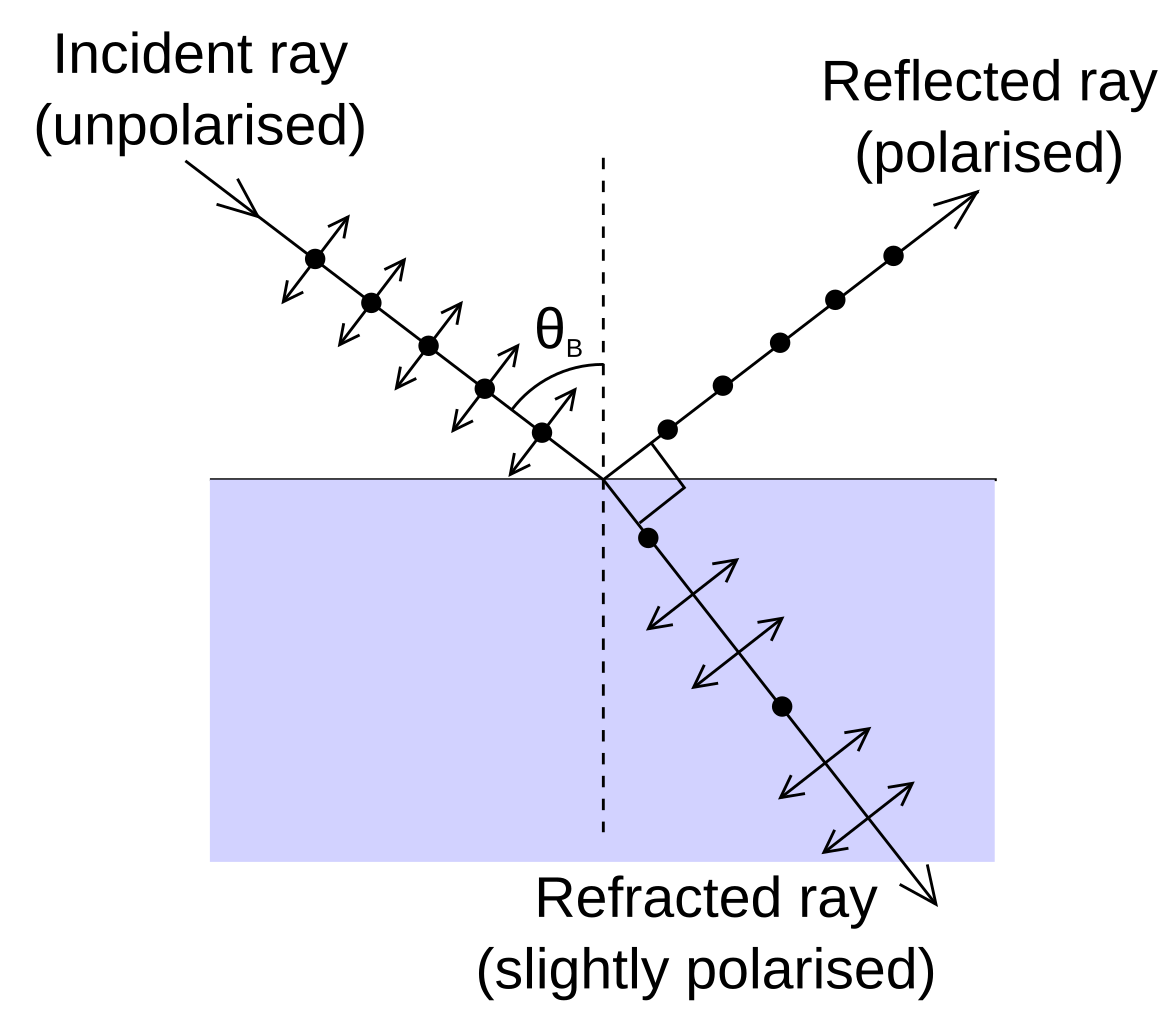
\includegraphics[width=0.25\textwidth]{slike/Brewsters-angle.svg.png}
    \caption{Brewster's angle }
    \label{fig:brewstr}
\end{figure}

\subsection{Linear polarization}
EM wave, shown on figure \ref{fig:linpol} is polarized linearly. 

\begin{figure}[h!]
    \centering
    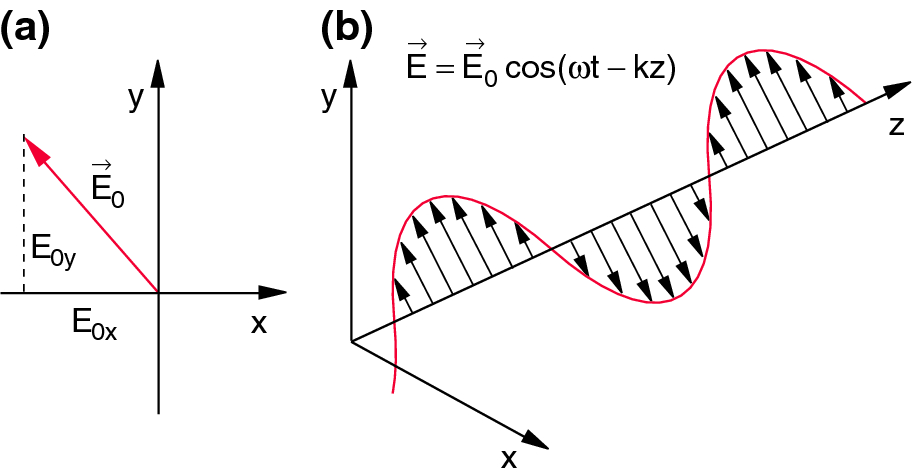
\includegraphics[width=0.5\textwidth]{slike/linpol.png}
    \caption{Linear polarization}
    \label{fig:linpol}
\end{figure}

Electric filed in $x,y$ directions can be described as:
\begin{align}
    E_x = E_{0x} cos(kz - \omega t)\\
    E_y = E_{0y} cos(kz - \omega t)
\end{align}
combined:
\begin{equation}
    E = (\vec{e}_x E_{0x} + \vec{e}_y E_{0y}) cos(kz - \omega t)
\end{equation}



\subsection{Circular polarization}
Circular polarization is shown on figure \ref{fig:cirpol}.
\begin{figure}[h!]
    \centering
    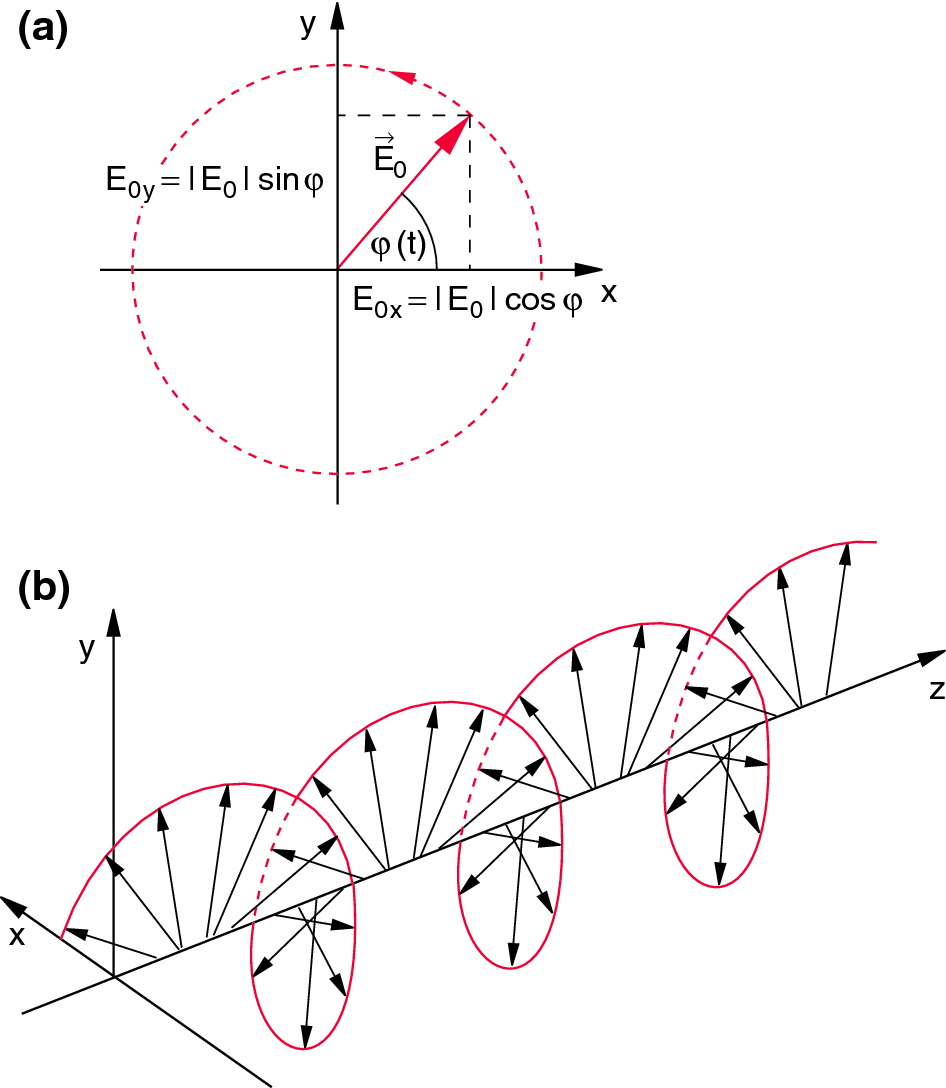
\includegraphics[width=0.35\textwidth]{slike/circpol.png}
    \caption{Circular polarization}
    \label{fig:cirpol}
\end{figure}

\begin{align}
    E_x = E_{0x} cos(kz - \omega t)\\
    E_y = E_{0y} cos(kz - \omega t + \frac{\pi}{2}) =  -E_{0y} cos(kz - \omega t)
\end{align}
combined (phase delay $\varphi = \frac{\pi}{2}$):
\begin{equation}
    \vec{E} = E_0 (\vec{e}_x cos(kz - \omega t) - \vec{e}_y sin(kz - \omega t))
\end{equation}

The delay $\varphi$, determines the way the light is polarized - clockwise or counterclockwise
polarization. 

When two EM-waves of different circular polarization are superimposed (interfere),
the result is linearly polarized light with the amplitude $2 E_0$.

\begin{align}
    \vec{E_1} = E_0 (\vec{e}_x cos(kz - \omega t) - \vec{e}_y sin(kz - \omega t))\\
    \vec{E_2} = E_0 (\vec{e}_x cos(kz - \omega t) + \vec{e}_y sin(kz - \omega t))\\
    \vec{E}_{res} = 2 E_0 \vec{e}_x cos(kz - \omega t)
\end{align}

In order to have circular polarization, $\varphi$ must be $0$\textdegree, $\pm 90$\textdegree, $180$\textdegree.

\subsection{Elliptical polarization}
When light polarization is \textbf{not} linear or circular, it is \textbf{elliptical}.
Such polarization is achieved when the phase difference of different waves is not $\varphi \ne 0, \pm \frac{1\pi}{2}
\pm \frac{2\pi}{2},\pm \frac{3\pi}{2}, \dots$. 

\subsection{Polarized and unpolarized light}
Any polarization can be seen as a superposition of two fundamental 
polarization types:
\begin{itemize}
    \item two orthogonal linear polarizations
    \item two counter-rotating circular polarizations
\end{itemize}

Unpolarized light contains waves polarized in different directions. Most light sources emit unpolarized light.

\textbf{Most lasers} emit \textbf{polarized} light due to their fundamental properties or design.
It is possible to rotate linear polarization, \textbf{without energy loss}, using a \textit{half-waveplate}. Converting circularly polarized light to linearly polarized light 
using a \textit{quarter-waveplate}.